%% The following is a directive for TeXShop to indicate the main file
%%!TEX root = diss.tex

\chapter{Theory}
\label{ch:Theory}

\section{Cherenkov Radiation}
\label{sec:cherenkov}
Although the speed of light in a vacuum is a constant $c$, when light passes through a medium with a refractive index of $n$, it will travel at the velocity $c/n$.
When a charged particle travels through a dielectric medium (known as a radiator) at a velocity greater than the speed of light in the medium, it will displace electrons, emitting photons radially at points along the particle's path. it will emit Cherenkov radiation \cite{cherenkov}.
If we define the particle velocity to be $v_p$ and $\beta = v_p / c$, then in a time $t$, the particle will travel a distance $\beta ct$.
In that same amount of time, the photons emitted in the radiator will have travelled a distance $(c/n)t$.
The geometry of this emission is shown in in Figure \ref{fig:cherenkov}.
This creates a wavefront of light emitted obeying the following relation:
\begin{equation}
    cos(\theta) = \frac{1}{\beta n}
    \label{eq:cherenkovAngle}
\end{equation}

\begin{figure}[]
\centering
\resizebox{0.8\textwidth}{!}{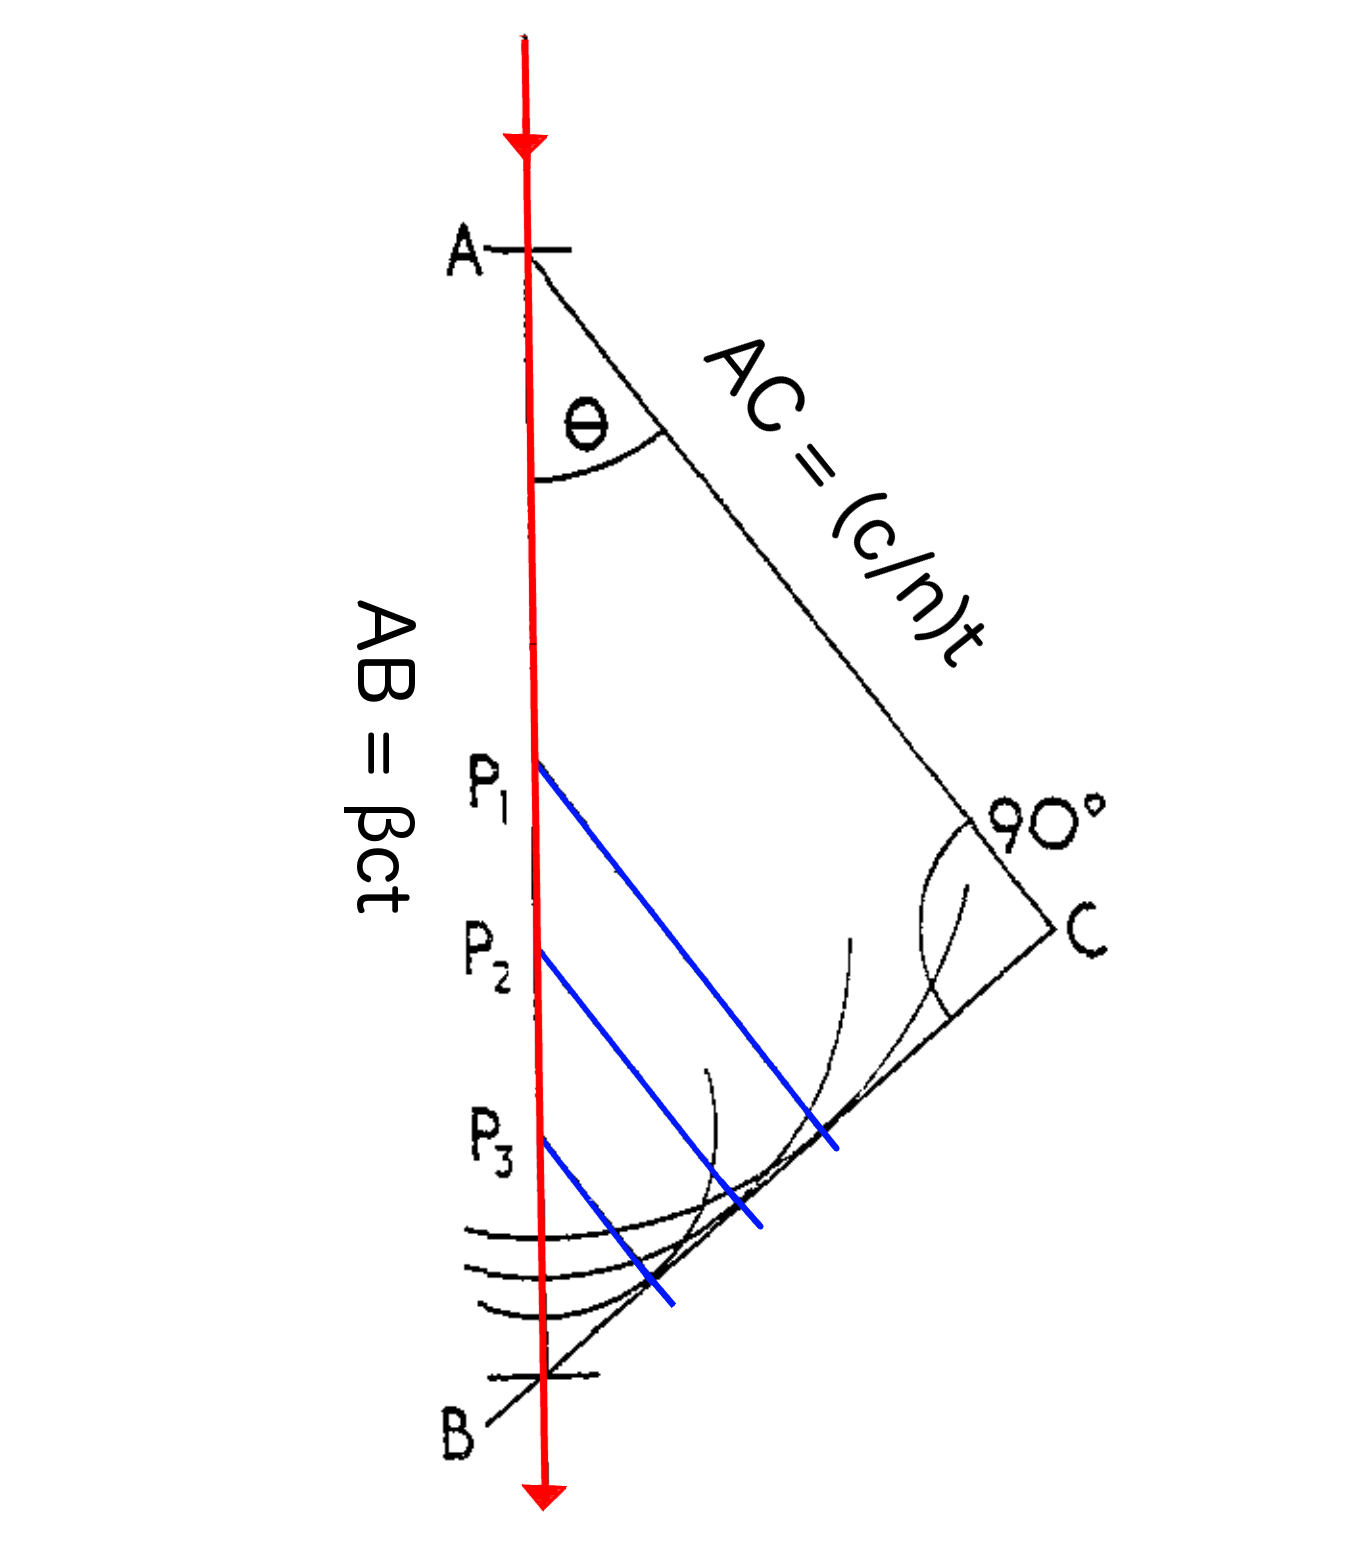
\includegraphics{./figs/cherenkovMod.png}}
\caption[Diagram showing the emission of Cherenkov radiation]{Diagram showing the emission of Cherenkov radiation, adapted from \cite{cherenkov}.
In this diagram, a particle travels along the vertical line from point A to point B.
Electromagnetic radiation is emitted at $P_1$, $P_2$, and $P_3$, each producing one of the curves shown.
It can be seen that these emissions all produce a wavefront along BC, giving a common angle of emission $\theta$.}
\label{fig:cherenkov} 
\end{figure}

The energy emitted via Cherenkov radiation by a particle of charge $q$ as it moves a distance $dl$ through a radiator is given by the Frank-Tamm formula \cite{frankTamm}:
\begin{equation}
    \label{eq:frankTamm}
    \frac{dW}{dl} = \frac{q^2}{c^2}\int_{\beta n > 1} \omega  \left(1 - \frac{1}{\beta^2n(\omega)^2}\right)d\omega
\end{equation}

In this formula, $\omega$ is the angular frequency of the light.
If we neglect the frequency dependence of the index of refraction, then we can use this equation to extract the expected number of photons emitted per length $dl$ over a range of frequencies from $\lambda_1$ to $\lambda_2$:

\begin{equation}
    \label{eq:photonNumber}
    \frac{dN}{dl}  = 2\pi\alpha q^2 \left(\frac{1}{\lambda_2} - \frac{1}{\lambda_1}
    \right)\left(1 - \frac{1}{\beta^2n^2}\right)
\end{equation}

Here, $\alpha$ is the fine structure constant ($\approx \frac{1}{137}$).



\section{Aerogel Ring Imaging Cherenkov Detectors}
\label{sec:ARICH}
The relationship between particle velocity through a radiator and photon angle of emission (Equation \ref{eq:cherenkovAngle}) can be exploited for particle identification.
An \ac{ARICH} detector consists of a silica aerogel radiator, and an array of \ac{PMT}s, which can detect Cherenkov radiation of charged particles passing through the aerogel.
Silica aerogel is a substance made of a network of silica (SiO$_2$) clusters interspersed with nanopores of air \cite{aerogelRefraction}.
During production, the refractive index of aerogel can be precisely tuned \cite{aerogelRefraction}, and the wavelength-dependency of the refractive index is understood \cite{aerogelWavelength}. 



High-velocity charged particles produced in the collision of the proton beam with a target will emit cones of Cherenkov radiation as they travel through the aerogel, leading to an elliptically shaped set of detected photons.
As the angle of emission depends on the velocity of a particle, the radii of the ellipses depend just on the velocity of the particle, the distance between the point of emission and the detector, and the angle of the incident charged particle.

At the time of this project, the aerogels available for use for EMPHATIC had indices of refraction of 1.035, 1.04, 1.045, and 1.05.
Looking at Equation \ref{eq:cherenkovAngle}, we see that with a lower index of refraction, the Cherenkov angle changes more rapidly with respect to particle velocity. 
A rapidly changing angle would allow for the velocity of a particle to be better resolved, and so the aerogel with an index of refraction of 1.035 was chosen to be used in the detector.

By averaging over several photons emitted by a single particle, we can increase our angular resolution.
With a thicker slab of aerogel, a charged particle travels a greater distance and is likely to emit a greater number of photons.
However, this means that the point of emission of the photon can vary more, reducing the angular resolution.
To combat this, \ac{ARICH} detectors can use two or more layers of aerogel with differing indices of refraction, with the layer closest to the detector having a higher index of refraction \cite{belleArich}.
The photons emitted in the first layer will be emitted at a smaller angle than those from the second layer, and ultimately arrive on the same ring on the photon detector array.
The Cherenkov radius of a photon emitted from a charged particle travelling directly downstream at a velocity $\beta$, through a layer of aerogel with an index of refraction $n$ and a distance $d$ from the detector plane is given by:

\begin{equation}
d\tan\left(\arccos\left(\frac{1}{\beta n}\right)\right)
\end{equation}

For EMPHATIC, the slabs of aerogel were chosen to be 2 cm thick, and the first layer was chosen to be placed with its centre at a distance of 20 cm from the photon detector plane.
If the first layer has an index of refraction of $n = 1.035$, then to most closely match the Cherenkov radius for a typical particle velocity of $\beta \approx 1$, the best available value for the index of refraction of a second layer of aerogel placed 18 cm upstream of the detector plane would be 1.045. 
Since the start of this project, an aerogel with an index of refraction of 1.03 has become available.
However, because this was not available earlier, all subsequent analysis assumes aerogel indices of 1.035 and 1.045.

The \ac{PMT}s used in the detectors function by creating a rapid cascade of electrons and a corresponding signal upon being struck by a photon.
The quantum efficiencies depend on the wavelength of the incident light, and are well-characterized by the manufacturer.
After each photon detection, there is some deadtime in which a PMT pixel cannot detect any other incident photons.
Thus when multiple Chernekov photons emitted during a single event strike the same PMT pixel, only one will be detected.

\section{Optical Effects in the Detector}
\label{sec:optics}
A number of optical effects complicate the distributions of photons emitted in an ARICH detector.
As photons travel through the layers of aerogel, they have some probability of interacting with the medium, either via absorption, or via scattering.
Because the pockets of air included in the aerogel are smaller than the wavelength of visible light, the dominant effect is Rayleigh scattering \cite{aerogelRefraction}. 
The probability that a photon  undergoes Rayleigh scattering is proportional to $\lambda^{-4}$, where $\lambda$ is the wavelength of the light.
The angular distribution of scattered photons is proportional to $1 + \cos^2(\theta)$ \cite{rayleigh}.

\section{Particle Identification}
\label{sec:particleIdentification}
In order to identify particles using the \ac{ARICH} detector, a particle likelihood method may be used \cite{richImpact, belleArich}.
For this method, we take the measured momentum of the particle, and determined the expected velocity for different candidate particles masses.
The candidate particles of interest for this study are protons, with a mass of 0.938 GeV/c$^2$, pions, with a mass of 0.140 GeV/c$^2$, and kaons, with a mass of 0.494 GeV/c$^2$\TODO{cite pdg}.
To calculate the velocity, we then use the following relativistic equation, assuming units where $c = 1$:

\begin{equation}
\label{eq:relMass}
 \beta = \sqrt{\frac{1}{1 +m^2 / p^2}}
\end{equation}

For each velocity hypothesis, we can run many Monte Carlo simulations of particles moving at that velocity, with the same measured initial trajectory as the input event data, and get the distribution of the resulting photons.
For each pixel of the detector, this procedure will give a value $\lambda_i(\beta)$, equal to the expected number of photons striking pixel $i$ in the detector due to a particle of velocity $\beta$. 

For a given experimental event, we will detect $N_i$ photons in each pixel $i$: because of the deadtime of the detector,  we just know whether $N_i = 0$ or $N_i > 0$.
If we assume that the number of photons detected by a PMT pixel is given by a Poisson distribution, then the probability that zero photons strike pixel $i$ is given by:
\begin{equation}
P_i(N_i=0; \beta) = e^{-\lambda_i(\beta)}
\end{equation}

 The probability that one or more photons strike pixel $i$ must then be:
\begin{equation}
P_i(N_i>1; \beta) = 1 - e^{-\lambda_i(\beta)}
\end{equation}

By multiplying the probabilities of getting the observed result in each pixel $i$ of the detector, we calculate the likelihood for that value of $\beta$:

\begin{equation}
L_\beta = \prod_{i}P_i(N_i; \beta)
\end{equation}

Because of the floating point errors that would inevitably be introduced by multiplying hundreds of numbers together, we instead can look at twice the negative log of the likelihood:

\begin{equation}
    \label{eq:log-likelihood}
    -2\ln(L_\beta) = -2\sum_i \ln(P_i(N_i; \beta))
\end{equation}

Because the log function is montonic, maximizing the likelihood function is equivalent to minimizing the negative log-likelihood.
%One potential downside to using the negative log-likelihood is that if some bin has a computed value $\lambda$ of 0, then the likelihood of the distribution becomes $-\infinity$. 
%Because this may lead to numerical problems, we may apply some additive smoothing.
For each event, the negative log-likelihood can be calculated for each particle hypothesis, and we can predict that each event was caused by the particle that minimizes the negative log-likelihood.



\endinput

Any text after an \endinput is ignored.
You could put scraps here or things in progress.
